\documentclass[final,12pt]{beamer}

\mode<presentation> {
  \usetheme{Custom}
}

\usepackage{times}
\usepackage{adjustbox}
\usepackage{algpseudocode}
\usepackage{amsmath,amsthm,amssymb,latexsym}
\usepackage[english]{babel}
\usepackage[orientation=portrait,size=a0,scale=1.4,debug]{beamerposter}
\usepackage{hyperref}

\boldmath
\hypersetup{
  colorlinks,
  linkcolor=,
  urlcolor=blue
}

\makeatletter
\renewcommand{\ALG@beginalgorithmic}{\small}
\makeatother

\title{Implementation of Cache Management Algorithms in DM-Cache}
\author{Jesus Ramos (jramo028@fiu.edu)}
\institute[FIU]{Florida International University}
\date{}

\begin{document}
\begin{frame}{}

  \begin{columns}

    \begin{column}{.33\linewidth}
      \begin{block}{\large Problem Statement}
      \end{block}
    \end{column}

    \begin{column}{.33\linewidth}
      \begin{block}{\large Current Solutions}
      \end{block}
    \end{column}

    \begin{column}{.33\linewidth}
      \begin{block}{\large Objectives}

        \begin{itemize}
          \item Make DM-Cache more flexible when it comes to cache management
          \item Allow for implementation of other cache management algorithms
          \item Update the existing code base to a more recent kernel
          \item Lower the memory footprint of DM-Cache
        \end{itemize}

      \end{block}
    \end{column}

  \end{columns}

  \begin{block}{\large Design and Implementation}

    \begin{columns}

      \begin{column}{.01\textwidth}
      \end{column}

      \begin{column}{.33\textwidth}
        \begin{algorithmic}
  \State $block \gets$ look-up requested block in $radix\_tree$
  \If {$block$ is not cached}
    \If {$cache$ is full}
      \State evict from tail of $lru\_list$
    \EndIf
    \State initialize new $block$
    \State insert $block$ into $radix\_tree$
  \EndIf
  \State move $block$ to head of $lru\_list$
\end{algorithmic}

        \centering \small Pseudo-code for DM-Cache using LRU (Least Recently
        Used) cache eviction algorithm
      \end{column}

      \begin{column}{.33\textwidth}
        \begin{algorithmic}
  \State $block \gets$ look-up requested block in $radix\_tree$
  \If {$block$ is not cached}
    \If {$cache$ is full}
      \State evict from tail of $lfu\_list$
    \EndIf
    \State initialize new $block$
    \State insert $block$ into $radix\_tree$
    \State insert $block$ at tail of $lfu\_list$ with $hit\_count$ of $1$
  \Else
    \State $block.hit\_count \gets block.hit\_count + 1$
    \State $next\_block \gets$ adjacent entry of $block$ from $lfu\_list$
    \If {$block.hit\_count \geq next\_block.hit\_count$}
      \State swap $block$ and $next\_block$ in place
    \EndIf
  \EndIf
\end{algorithmic}


        \centering \small Pseudo-code for DM-Cache using LFU (Least Frequently
        Used) cache eviction algorithm
      \end{column}

      \begin{column}{.33\textwidth}
      \end{column}

    \end{columns}

  \end{block}

  \begin{columns}

    \begin{column}{.5\linewidth}
      \begin{block}{\large Screenshots}
        \centering
        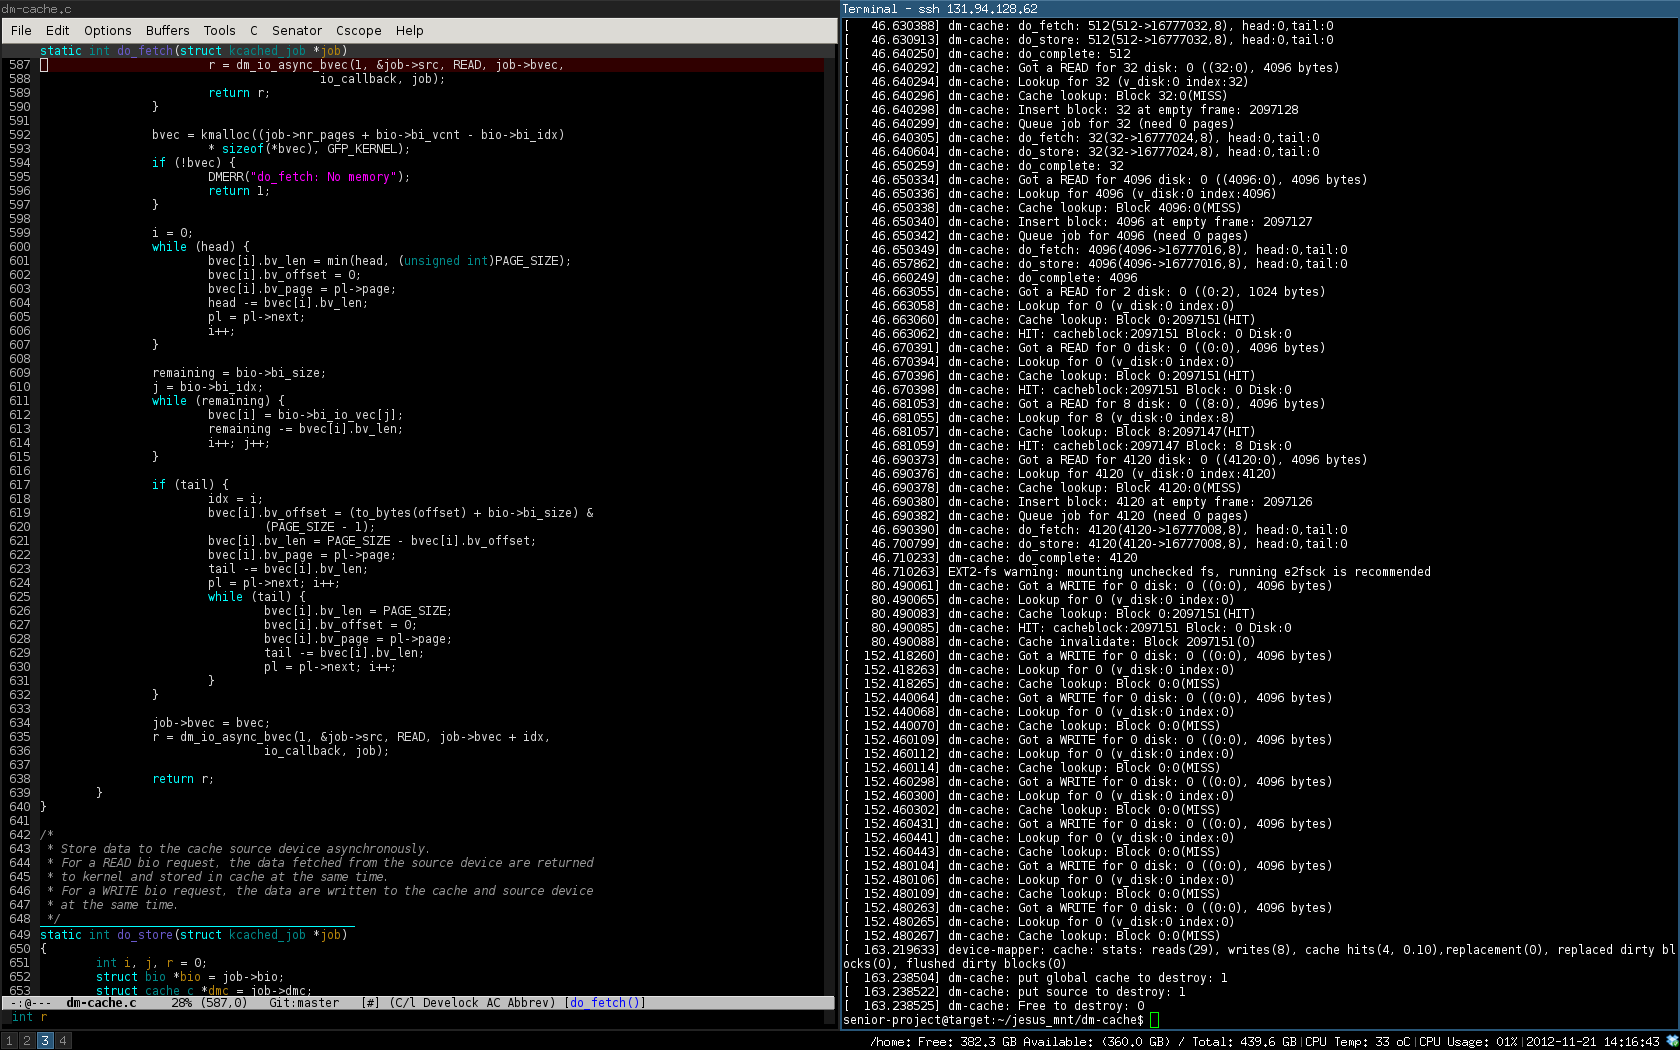
\includegraphics[width=.97\textwidth]{../images/screenshot.png}
      \end{block}
    \end{column}

    \begin{column}{.5\linewidth}
      \begin{block}{\large Testing}

        Testing was done using a virtual machine using an 8GB cache size. To
        exercise the cache eviction algorithms a test file size of 16GB was
        used. The tests that were performed were sequential writes, random
        writes, sequential reads, and random reads all using a 16GB file. To
        test that the cache was not losing or corrupting any blocks an original
        copy of the file was kept and the \texttt{diff} utility was run to check
        for inconsistencies.

        \vspace{\baselineskip}

        The code for this project can be found at:
        \url{https://github.com/jesus-ramos/senior-project}

        More information on DM-Cache can be found at:
        \url{https://github.com/mingzhao/dm-cache} \\
        and at: \\
        \url{http://visa.cs.fiu.edu/}

      \end{block}
    \end{column}

  \end{columns}

  % unneeded for now
  % \begin{block}{\large References}
  % \end{block}

\end{frame}
\end{document}